%%%%%%%%%%%%%%%%%%%%%%%%%%%%%%%%%%%%%%%%%%%%%%%%%%%%%%%%%%%%%%%%%%%%%%%%%%%%%%%%%%
\begin{frame}[fragile]\frametitle{}
\begin{center}
{\Large Theory Behind Rasa Platform}

{\tiny (Ref: Conversational AI:Building clever chatbots - Tom Bocklisch and Deprecating the state machine: building conversational AI with the Rasa stack - Justina Petraitytė) }

\end{center}
\end{frame}

%%%%%%%%%%%%%%%%%%%%%%%%%%%%%%%%%%%%%%%%%%%%%%%%%%%%%%%%%%%%%%%%%%%%%%%%%%%%%%%%%%
\begin{frame}[fragile]\frametitle{}
\begin{center}
{\Large NLU}

\end{center}
\end{frame}

%%%%%%%%%%%%%%%%%%%%%%%%%%%%%%%%%%%%%%%%%%%%%%%%%%%%%%%%%%%
 \begin{frame}[fragile]\frametitle{NLU Training}
 ``train'' function iterates through the pipeline and performs the NLP tasks
\begin{itemize}
\item The preprocessing step: Where the data is transformed to extract the required information. Eg. SpacyTokenizer, SpacyFeaturizer
\item Entity Extractor \& Intent Classifier: The preprocessed data is used to create the ML models that perform intent classification and entity extraction. NER\_CRF EntityExactor, SklearnIntentClassifier
\item Persistence : Storing the result
\end{itemize}
\end{frame}

%%%%%%%%%%%%%%%%%%%%%%%%%%%%%%%%%%%%%%%%%%%%%%%%%%%%%%%%%%%
\begin{frame}[fragile]\frametitle{Natural Language Understanding (NLU)}

Goal: create structured data

\begin{center}
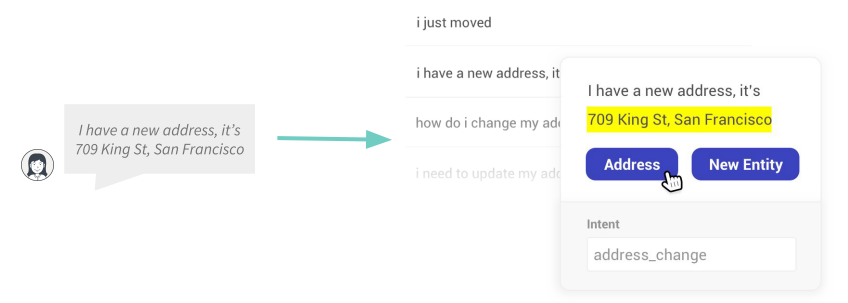
\includegraphics[width=\linewidth]{rasa15}
\end{center}


\end{frame}


%%%%%%%%%%%%%%%%%%%%%%%%%%%%%%%%%%%%%%%%%%%%%%%%%%%%%%%%%%%
\begin{frame}[fragile]\frametitle{Intent Classification}

\begin{center}
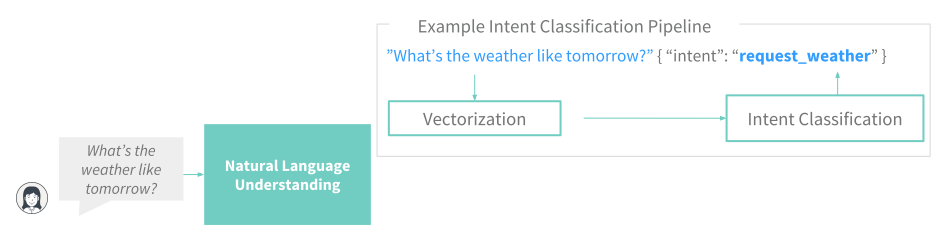
\includegraphics[width=\linewidth]{rasa16}
\end{center}


\end{frame}

%%%%%%%%%%%%%%%%%%%%%%%%%%%%%%%%%%%%%%%%%%%%%%%%%%%%%%%%%%%
\begin{frame}[fragile]\frametitle{Intent Classification}

\begin{center}
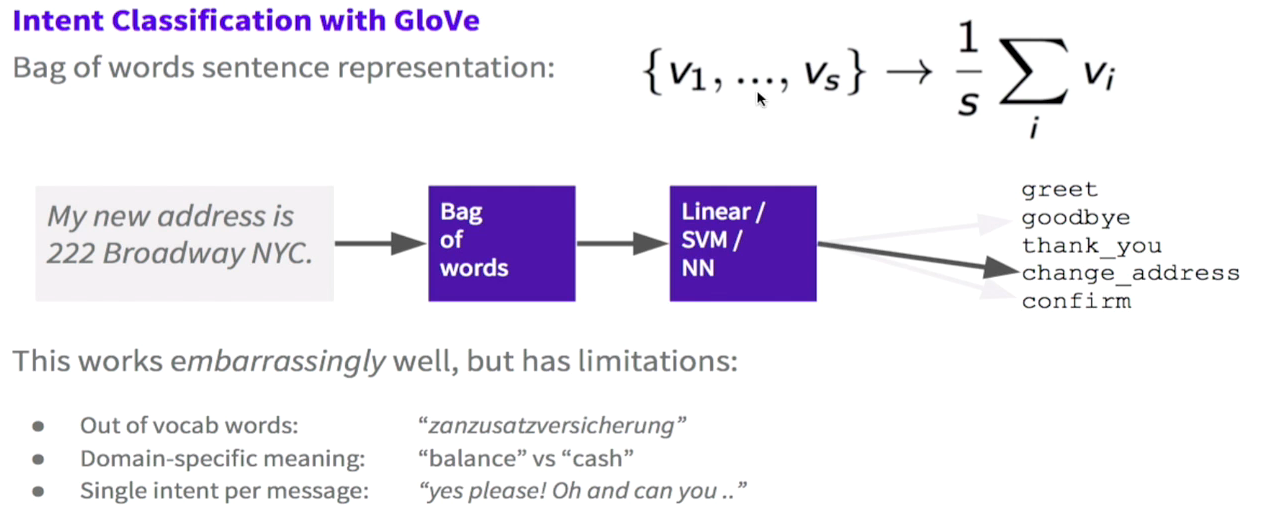
\includegraphics[width=\linewidth]{rasa17a}
\end{center}

\begin{itemize}
\item Get word embeddings of each word, form sentence embeddings by averaging, run a classifier to find max probability intent.
\item Classifier does not matter much but the quality of embedding does.
\item Need domain specific vocab!!
\end{itemize}

\end{frame}


%%%%%%%%%%%%%%%%%%%%%%%%%%%%%%%%%%%%%%%%%%%%%%%%%%%%%%%%%%%
\begin{frame}[fragile]\frametitle{Entity Extraction}

\begin{center}
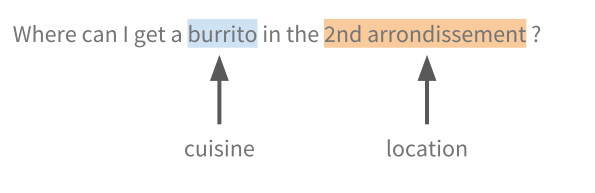
\includegraphics[width=\linewidth]{rasa18}
\end{center}

\begin{itemize}
\item Can be done in phases.
\item First, have a Binary classifier just to detect if the sentence has entities or not.
\item Next, it would be multi class classifier to find WHICH entity is there?
\item NER with Conditional Random Fields
\end{itemize}
\end{frame}


%%%%%%%%%%%%%%%%%%%%%%%%%%%%%%%%%%%%%%%%%%%%%%%%%%%%%%%%%%%
\begin{frame}[fragile]\frametitle{NLU Full Workflow}


\begin{center}
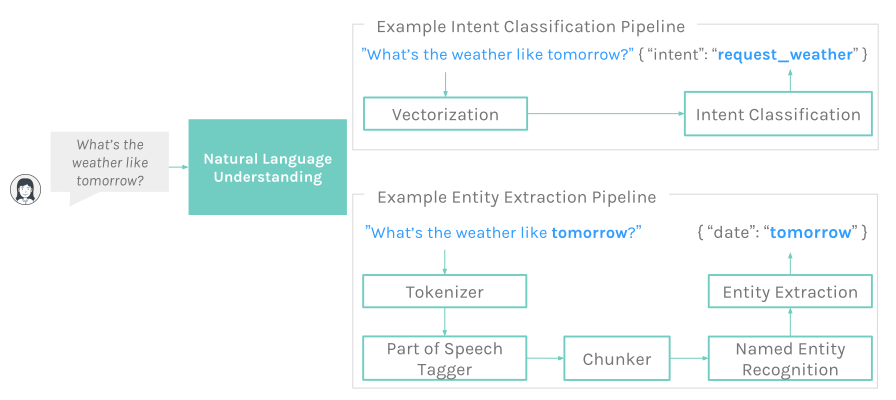
\includegraphics[width=\linewidth]{rasa10}
\end{center}

\end{frame}

%%%%%%%%%%%%%%%%%%%%%%%%%%%%%%%%%%%%%%%%%%%%%%%%%%%%%%%%%%%
\begin{frame}[fragile]\frametitle{NLU is Hard}

Especially negations:

\begin{center}
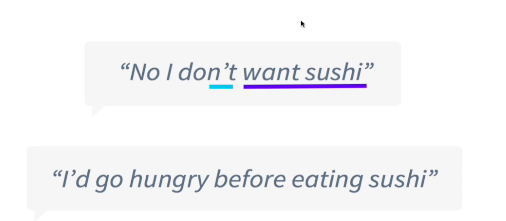
\includegraphics[width=0.6\linewidth]{rasa21}
\end{center}

\begin{itemize}
\item Both the sentences have same meaning, but how to detect!!
\item First one is easy, find the negative "not" (LSTM can look for these associations), but how about the second one.
\end{itemize}

\end{frame}

%%%%%%%%%%%%%%%%%%%%%%%%%%%%%%%%%%%%%%%%%%%%%%%%%%%%%%%%%%%
\begin{frame}[fragile]\frametitle{}

NLU is Impossible (\textit{mushkil hi nahi, na mumkin hai})

Some hopes: better (sentence level) embeddings.
\end{frame}

%%%%%%%%%%%%%%%%%%%%%%%%%%%%%%%%%%%%%%%%%%%%%%%%%%%%%%%%%%%%%%%%%%%%%%%%%%%%%%%%%%
\begin{frame}[fragile]\frametitle{}
\begin{center}
{\Large Core}

\end{center}
\end{frame}

%%%%%%%%%%%%%%%%%%%%%%%%%%%%%%%%%%%%%%%%%%%%%%%%%%%%%%%%%%%
\begin{frame}[fragile]\frametitle{Rasa Core: Getting Rid of State Machines}
The main idea behind Rasa Core: 
\begin{itemize}
\item Thinking of conversations as a flowchart is WRONG
\item Implementing conversations as state machine is WRONG
\item Its had to come up with ALL possible conversations upfront and explicitly.
\end{itemize}

\end{frame}

%%%%%%%%%%%%%%%%%%%%%%%%%%%%%%%%%%%%%%%%%%%%%%%%%%%%%%%%%%%
 \begin{frame}[fragile]\frametitle{State Machines}
Say, for Insurance Purchase bot, the state machine could be:

\begin{center}
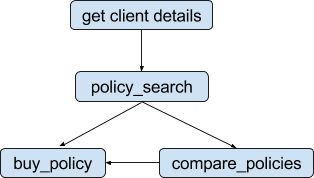
\includegraphics[width=0.5\linewidth,keepaspectratio]{chatbot55}

\end{center}

It can take any branch!! What's more likely at a particular state, can be learnt by past data only, ie Machine Learning.
\end{frame}


%%%%%%%%%%%%%%%%%%%%%%%%%%%%%%%%%%%%%%%%%%%%%%%%%%%%%%%%%%%
 \begin{frame}[fragile]\frametitle{State Machines}
State Machines are infeasible

\begin{center}
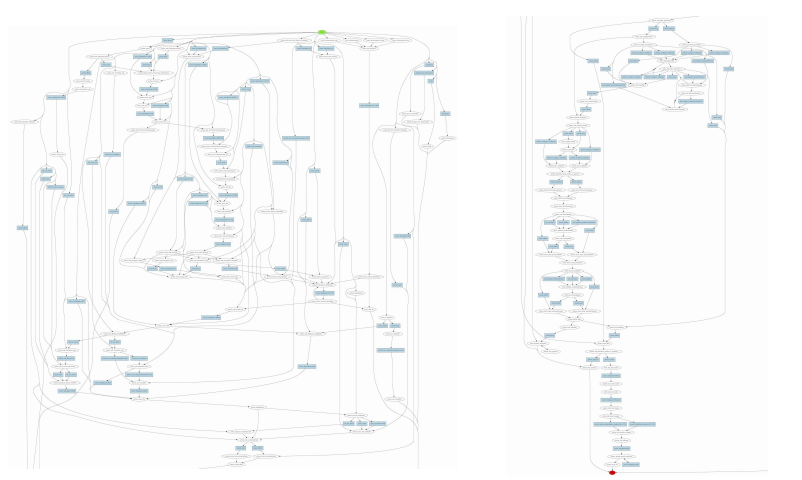
\includegraphics[width=0.9\linewidth,keepaspectratio]{chatbot25}

\end{center}

\end{frame}


%%%%%%%%%%%%%%%%%%%%%%%%%%%%%%%%%%%%%%%%%%%%%%%%%%%%%%%%%%%
 \begin{frame}[fragile]\frametitle{State Machines}
State Machines don't scale

\begin{center}
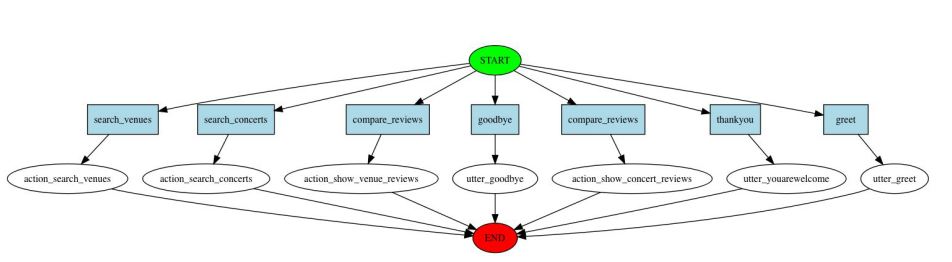
\includegraphics[width=0.9\linewidth,keepaspectratio]{chatbot26}

\end{center}

\end{frame}


%%%%%%%%%%%%%%%%%%%%%%%%%%%%%%%%%%%%%%%%%%%%%%%%%%%%%%%%%%%
 \begin{frame}[fragile]\frametitle{Why Machine Learning?}
\begin{center}
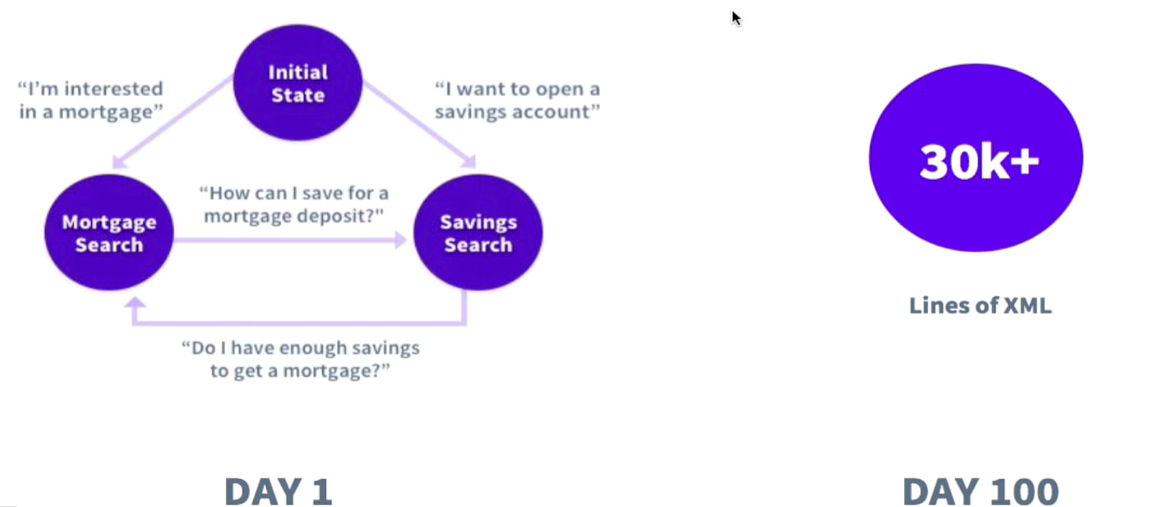
\includegraphics[width=\linewidth,keepaspectratio]{chatbot36}

\end{center}

Example above is showing real numbers!!


{\tiny (Ref: Building Conversational AI w Rasa Stack - Alan Nichol at PyBay2018)}

\end{frame}


%%%%%%%%%%%%%%%%%%%%%%%%%%%%%%%%%%%%%%%%%%%%%%%%%%%%%%%%%%%
 \begin{frame}[fragile]\frametitle{Rasa Core Approach}
\begin{itemize}
\item Machine learning will be predicting the next action.
\item But new approach cannot change radically an existing process: If you want a freaking pizza, you MUST tell a chatbot what type of base, what toppings you want and where you want it delivered.
\item 
But let's be clever about it, there are always exceptions like in the case of pizza: ALLERGIES !! something unexpected. 
\item Sure you can define a logic around but how many such logic are you going to code each day.
\item Keep in mind, Rasa core is not changing your process neither the machine is generating responses, it just allows you to handle exceptions better. Your rules still rule
\end{itemize}

\tiny{(Ref: Contextual Conversational Engine— The Rasa Core Approach: Part 1 - Souvik Ghosh)}

\end{frame}

%%%%%%%%%%%%%%%%%%%%%%%%%%%%%%%%%%%%%%%%%%%%%%%%%%%%%%%%%%%
 \begin{frame}[fragile]\frametitle{Example: Ordering Food}
 
 Let's build the different states
 
\begin{center}
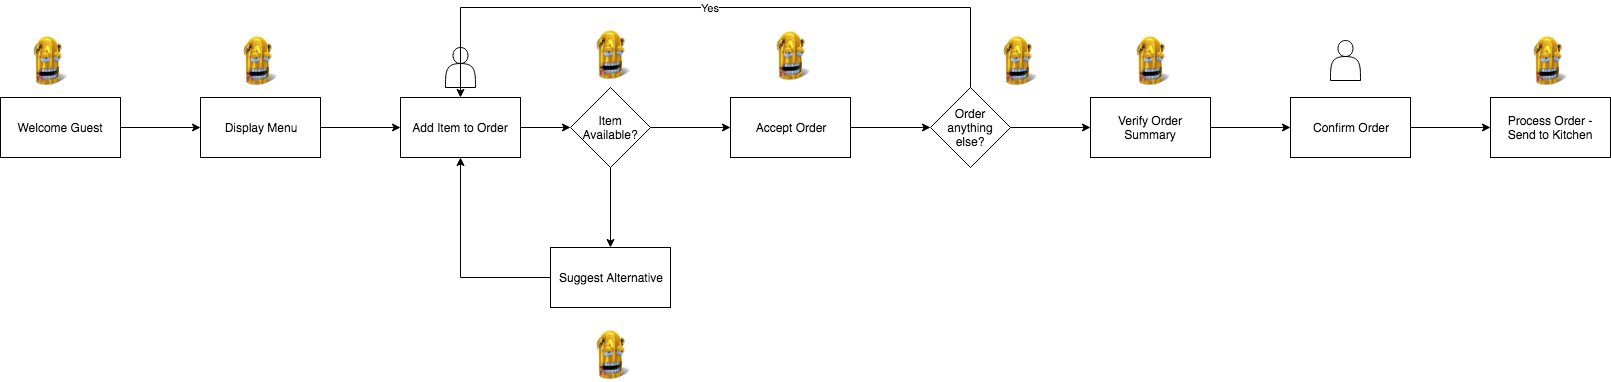
\includegraphics[width=\linewidth,keepaspectratio]{chatbot33}

\end{center}

\begin{itemize}
\item As you can already see, a simple ordering conversation is quite complicated already, 
\item Covered one of the exceptions, where a given item is not available , the bot can suggest some alternatives. 
\item There could many such alternatives and how do we deal with item
\end{itemize}


\tiny{(Ref: Contextual Conversational Engine— The Rasa Core Approach: Part 1 - Souvik Ghosh)}

\end{frame}

%%%%%%%%%%%%%%%%%%%%%%%%%%%%%%%%%%%%%%%%%%%%%%%%%%%%%%%%%%%
 \begin{frame}[fragile]\frametitle{Training Steps}
 

\begin{center}
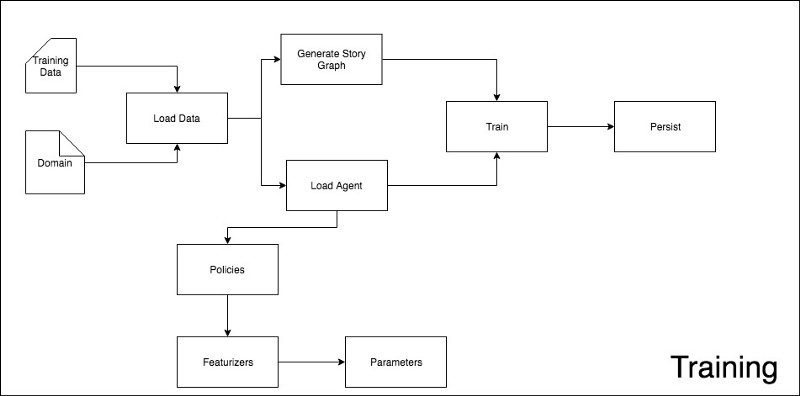
\includegraphics[width=0.8\linewidth,keepaspectratio]{chatbot34}

\end{center}

\begin{itemize}
\item Training Data: This is essentially all the stories where you typically define what is a normal conversation for your process.
\item Domain basically determines what your chatbot should understand, what the chatbot can do and what kind of information is necessary for your chatbot's context so it understands the user better. 
\end{itemize}


\tiny{(Ref: Contextual Conversational Engine— The Rasa Core Approach: Part 1 - Souvik Ghosh)}

\end{frame}

%%%%%%%%%%%%%%%%%%%%%%%%%%%%%%%%%%%%%%%%%%%%%%%%%%%%%%%%%%%
 \begin{frame}[fragile]\frametitle{Training Steps}
 

\begin{center}
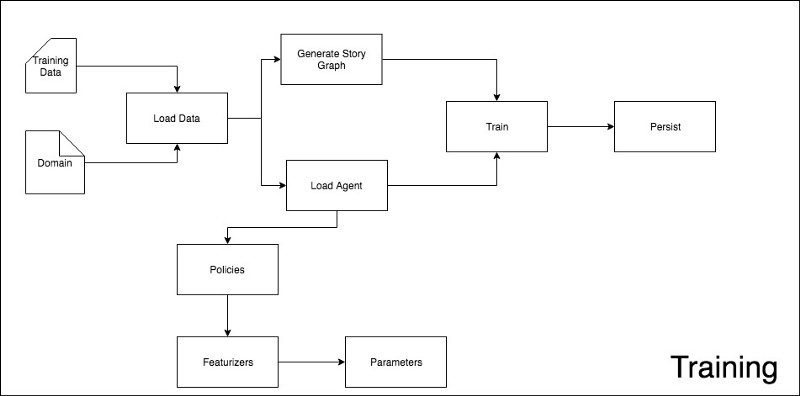
\includegraphics[width=0.8\linewidth,keepaspectratio]{chatbot34}

\end{center}

\begin{itemize}
\item Load Agent: Agent(or the bot) is first loaded with some parameters that determines how the training data will be converted into features for training the agent. ne really important parameter is ``Policy''
\item A policy is what will define what is going to be the next action. As Rasa core is open-source, you can indeed create your own policy but let's get the basics right and see what are the already available policies that are used by default.
\end{itemize}


\tiny{(Ref: Contextual Conversational Engine— The Rasa Core Approach: Part 1 - Souvik Ghosh)}

\end{frame}

%%%%%%%%%%%%%%%%%%%%%%%%%%%%%%%%%%%%%%%%%%%%%%%%%%%%%%%%%%%
 \begin{frame}[fragile]\frametitle{Prediction Process}
 

\begin{center}
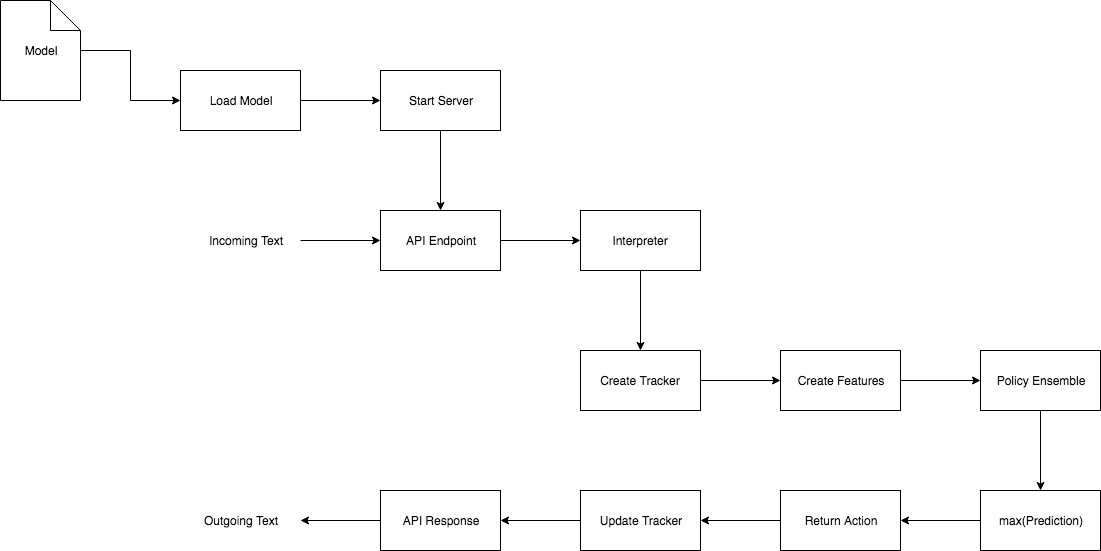
\includegraphics[width=0.8\linewidth,keepaspectratio]{chatbot35}

\end{center}

\begin{itemize}
\item Load Model in memory before serving using a Server( Flask ) and exposing an endpoint related to a particular channel, in our case we will deal with a REST API.
\item Interpreter is able to read the raw text coming in from user and throw out the intention of the user along with some meaning entities, these entities which we are saving as slots that will drive the conversation.
\end{itemize}


\tiny{(Ref: Contextual Conversational Engine— The Rasa Core Approach: Part 1 - Souvik Ghosh)}

\end{frame}

%%%%%%%%%%%%%%%%%%%%%%%%%%%%%%%%%%%%%%%%%%%%%%%%%%%%%%%%%%%
 \begin{frame}[fragile]\frametitle{Prediction Process}
 

\begin{center}
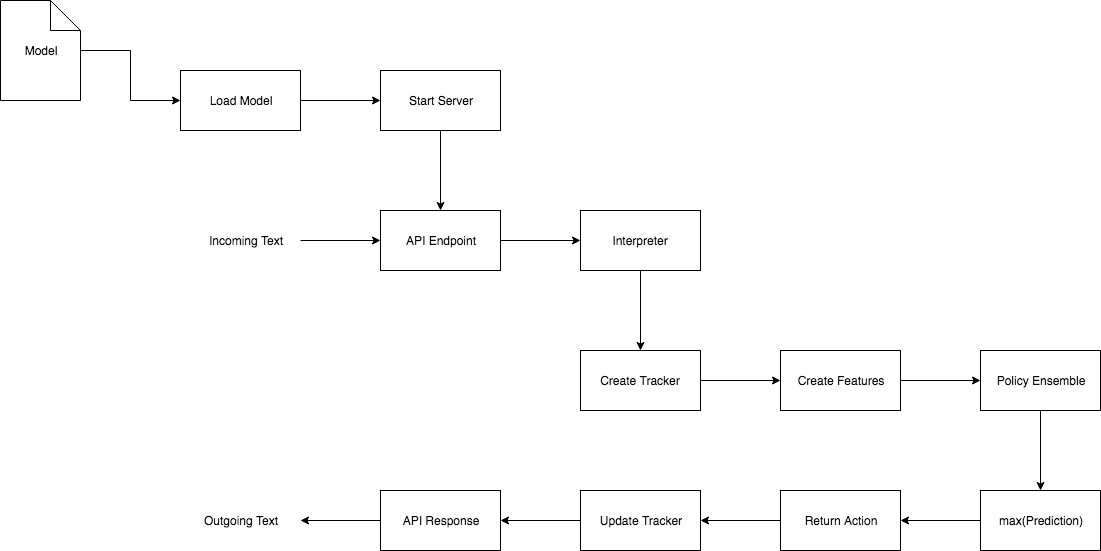
\includegraphics[width=0.8\linewidth,keepaspectratio]{chatbot35}

\end{center}

\begin{itemize}
\item CreateOrUpdate Tracker: If this is the first message of the conversation, rasa core will create a tracker object with the key ``sender\_id'' which is the incoming identifier of the user. Tracker object is usually stored in a tracker\_store which is by default is in InMemory.
\item Features are generated from contents of the tracker based on the policy 
\item Features will given to the policy ensemble which will determine the final outcome.
\end{itemize}


\tiny{(Ref: Contextual Conversational Engine— The Rasa Core Approach: Part 1 - Souvik Ghosh)}

\end{frame}

%%%%%%%%%%%%%%%%%%%%%%%%%%%%%%%%%%%%%%%%%%%%%%%%%%%%%%%%%%%
 \begin{frame}[fragile]\frametitle{Prediction Process}
 

\begin{center}
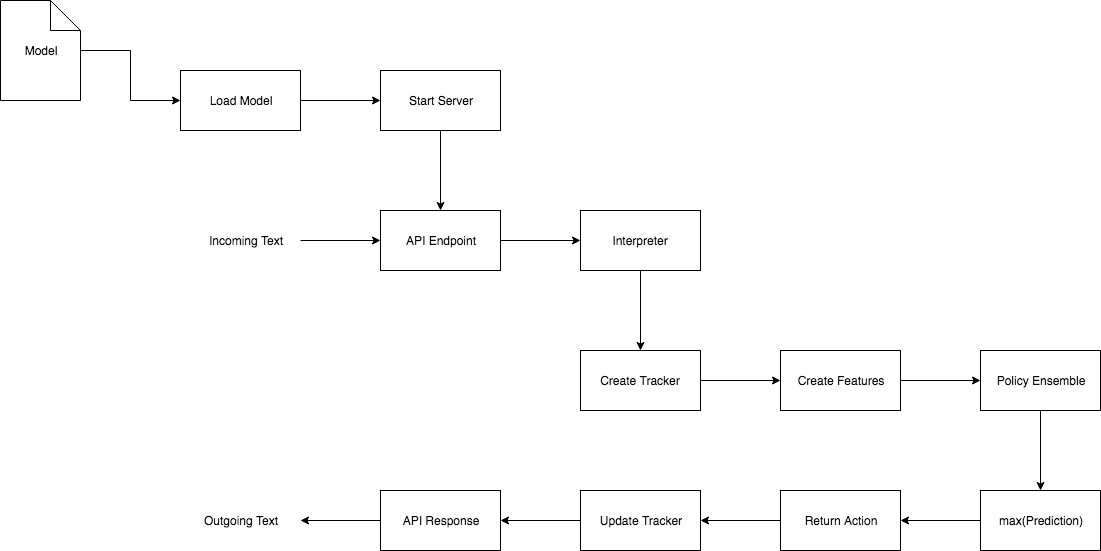
\includegraphics[width=0.8\linewidth,keepaspectratio]{chatbot35}

\end{center}

\begin{itemize}
\item PolicyEnsemble: Since, we have trained different policies, when it comes to predicting the next action, each of these policies will provide a score for the particular action. 
\item Then there is a max taken from all scores given by every policy and whichever wins, will be the next action
\end{itemize}


\tiny{(Ref: Contextual Conversational Engine— The Rasa Core Approach: Part 1 - Souvik Ghosh)}

\end{frame}

%%%%%%%%%%%%%%%%%%%%%%%%%%%%%%%%%%%%%%%%%%%%%%%%%%%%%%%%%%%
 \begin{frame}[fragile]\frametitle{Prediction Process}
 

\begin{center}
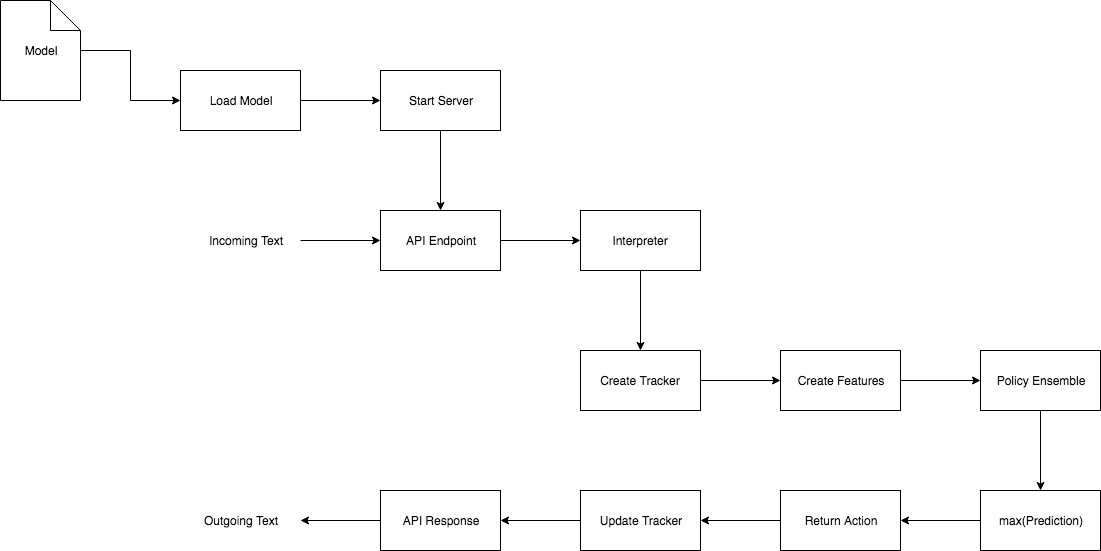
\includegraphics[width=0.8\linewidth,keepaspectratio]{chatbot35}

\end{center}

\begin{itemize}
\item Update Tracker: Once you have the action predicted, you will need to update the tracker for the next turn
\item ExecuteAction: Now you will be finally executing your action, be it an API call or a message sent back to the user
\end{itemize}


\tiny{(Ref: Contextual Conversational Engine— The Rasa Core Approach: Part 1 - Souvik Ghosh)}

\end{frame}


%%%%%%%%%%%%%%%%%%%%%%%%%%%%%%%%%%%%%%%%%%%%%%%%%%%%%%%%%%%
 \begin{frame}[fragile]\frametitle{Machine Learning Workflow}
\begin{center}
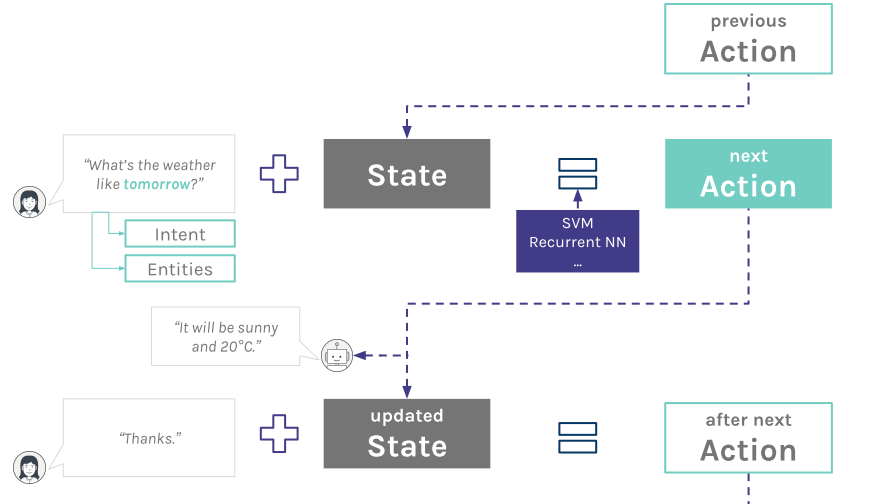
\includegraphics[width=\linewidth,keepaspectratio]{chatbot27}

\end{center}

\end{frame}
%%%%%%%%%%%%%%%%%%%%%%%%%%%%%%%%%%%%%%%%%%%%%%%%%%%%%%%%%%%
\begin{frame}[fragile]\frametitle{Dialogue Handling (Core)}


\begin{center}
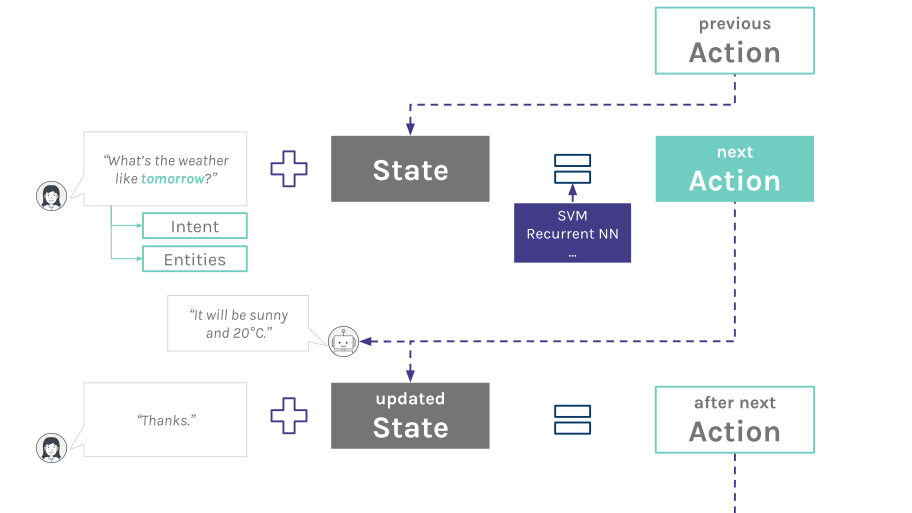
\includegraphics[width=\linewidth]{rasa11}
\end{center}


\end{frame}

%%%%%%%%%%%%%%%%%%%%%%%%%%%%%%%%%%%%%%%%%%%%%%%%%%%%%%%%%%%
\begin{frame}[fragile]\frametitle{Detailed Dialogue Handling (Core)}


\begin{center}
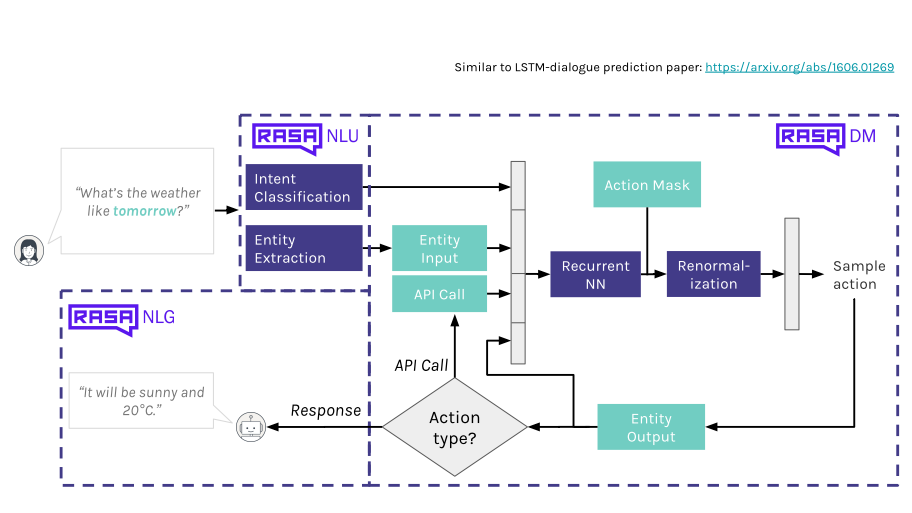
\includegraphics[width=\linewidth]{rasa12}
\end{center}


\end{frame}
